%\motto{Use the template \emph{chapter.tex} to style the various elements of your chapter content.}


\chapter{Quantenhardware}
\label{hardware} % Always give a unique label
% use \chaptermark{}
% to alter or adjust the chapter heading in the running head

\chapterauthor{Dennis Hülsken, Jakob Krumke, Marc Meyer, Daniel Roth, Tom Slatosch}

\abstract{some abstract}

\section{Die verschiedenen Quanten Hardwareplattformen}
Die Realisierung von Quantencomputern basiert wie beschrieben auf verschiedenen physikalischen Plattformen, die sich durch ihre spezifischen Qubit-Implementierungen, Steuerungsmechanismen und Anwendungsbereiche unterscheiden. Es wird zwischen zwei verschiedenen übergeordneten Hardwareplattformen unterschieden:
\begin{itemize}
    \item Festkörperplattformen, welche meistens aus Supraleiter oder Diamant basierte NV-Zentren bestehen
    \item Atomare Plattformen, welche auf Ionen oder Photonen basieren
\end{itemize}
Diese Unterschiede in Plattformen wirken sich erheblich auf die Skalierbarkeit, die Kohärenzzeiten und die potenziellen Anwendungsfelder bei Quantencomputer aus. Für beide Hauptplattformen existieren weitere Plattformen, wie z. B. Neutralatom-fallen oder Quanten-Punkte, sind jedoch aktuell nicht so forschungsrelevant wie die vorgestellten Plattformen.

\subsection{Unterschied atomare und Festkörper Plattformen}

Wie im vorherigen Kapitel vorgestellt, existieren in der Benutzung der Hauptplattformen Unterschiede.
\begin{itemize}
    \item Genaue Vorstellung Atomare Plattformen
    \item Genaue Vorstellung Festkörper Plattformen
\end{itemize}

Die folgende Tabelle gibt einen kompakten Überblick über die wichtigsten Eigenschaften beider Plattformarten:

\begin{tabular}{ |p{4cm}|p{5cm}|p{5cm}|  }
 \hline
 \textbf{Aspekt}& \textbf{Atomare Plattformen} & \textbf{Festkörperplattformen}\\
 \hline
 \textbf{Beispiele}   & Ionenfallen-Qubits, neutrale Atome    &Supraleitende Qubits, Halbleiter-Spin-Qubits, NV-Zentren\\
 \textbf{Qubit-Implementierung}&   Nutzung einzelner Atome oder Ionen als Qubits	  & Nutzung elektronischer oder magnetischer Zustände
\\
 \textbf{Kohärenzzeiten} &Sehr lang (Sekunden bis Minuten)	 & Kürzer (Mikrosekunden bis Millisekunden)
\\
 \textbf{Steuerung}    &Laser- und Mikrowellensteuerung	 & Mikrowellen- oder elektrischer Steuerung
\\
 \textbf{Herstellung}&   Aufwändige atomare Präparation und Kühlung	  & Integration in Halbleiterfertigung
\\
 \textbf{Skalierbarkeit}& Schwierig durch komplexe Fallen- oder Lasersysteme	  & Gut integrierbar, skalierbar
   \\
 \textbf{Anwendungen}& Präzise Quantenlogik, Metrologie, Quantensimulationen	  & Algorithmische Anwendungen, Quantenchemie, Optimierung
\\
 \hline
\end{tabular}

\section{Supraleitende Qubits}
Supraleitende Quantencomputer nutzen die Prinzipien der Quantenmechanik und die einzigartigen Eigenschaften von Supraleitern, um Quantenberechnungen durchzuführen. Diese Systeme sind darauf ausgelegt, komplexe Aufgaben in Bereichen wie Quantenchemie, Simulation, Kryptographie und Optimierung zu bewältigen, was ihnen potenzielle Vorteile gegenüber klassischen Systemen verschafft. Die Realisierung dieser Rechenvorteile hängt jedoch von der effizienten und skalierbaren Ausführung von Quantenprogrammen auf robuster Hardware ab, die für Quantenoperationen konzipiert ist.
\subsection{physikalisches Prinzip supraleitende qubits}
\subsection{Implementierung von Quantenlogik}
\subsubsection{Grundlegende Prinzipien und Typen}
Die fundamentalen Einheiten der Quanteninformation in supraleitenden Systemen sind supraleitende Qubits, die als künstliche Atome mit quantisierten Energieniveaus fungieren. Diese Qubits werden typischerweise aus supraleitenden Schaltkreisen gefertigt, die Materialien wie Aluminium oder Niob verwenden und bei extrem niedrigen Temperaturen, nahe dem absoluten Nullpunkt (ca. 15 Millikelvin), betrieben werden(The ultimate Guide to Superconducting Quantum Computers, 2025). Die Supraleitung, die bei diesen Temperaturen erreicht wird, gewährleistet einen widerstandslosen Stromfluss, was für die Aufrechterhaltung der Kohärenz der Qubits und ihrer Quantenzustände unerlässlich ist.
\\\\
Ein supraleitendes Qubit besteht häufig aus einem Induktor und einem Kondensator (LC-Oszillator), die durch einen Josephson-Kontakt verbunden sind. Der Josephson-Kontakt ist ein entscheidendes nichtlineares Element, das eine Anharmonizität in das Energiespektrum des Schaltkreises einführt. Diese Anharmonizität ist von größter Bedeutung, da sie sicherstellt, dass nur die beiden niedrigsten Energiezustände - der Grundzustand 0 and der erste angeregte Zustand 1 - als Qubit-Zustände dienen. Ohne diese Nichtlinearität würde der Quanten-LC-Schaltkreis als einfacher harmonischer Oszillator mit äquidistanten Energieniveaus fungieren, wodurch eine isolierte Zwei-Niveau-System-Nutzung als Qubit unmöglich wäre. Die präzise technische Gestaltung des Josephson-Kontakts und die Auswahl des supraleitenden Materials sind daher nicht nur Fertigungsdetails, sondern grundlegend für die Schaffung eines stabilen und adressierbaren Zwei-Niveau-Systems. Sie bestimmen die grundlegenden Eigenschaften des Qubits wie Anharmonizität, Kohärenzzeit und Rauschresistenz, die für zuverlässige Quantenoperationen unerlässlich sind. Die Betriebsumgebung von supraleitenden Quantencomputern erfordert extrem niedrige Temperaturen, typischerweise im Bereich von 10 bis 20 Millikelvin(mK). Um diese Temperaturen zu erreichen, werden komplexe Kühlsysteme, meist Dilution Refridgerators, benötigt. Um eine solch extreme Kühlung zu ermöglichen, wird die Phasenmischung von Helium-3 und Helium-4 verwendet. Eine genauere Beschreibung zum Aufbau der Kühlsysteme und deren Funktionsweise sowie aktuelle Modelle, sind im Kapitel 1.2.4 zu finden.
\\\\
Der am häufigsten verwendete Qubit-Typ, bei supraleitenden Quantencomputern, ist das Transmon-Qubit. Dieser Transmon-Qubit weißt einen spezifische Hardwareaufbau auf. Er ist eine Weiterentwicklung des Cooper-Pair-Box-Qubits und besteht im Wesentlichen aus einem Josephson-Kontakt, der parallel zu einem relativ großen Shunt-Kondensator geschaltet ist. Dieser Kondensator, oft in einer "Kreuz"-Form (bekannt als Xmon), ist entscheidend, da er die Empfindlichkeit des Qubits gegenüber Ladungsrauschen drastisch reduziert und somit längere Kohärenzzeiten ermöglicht. Die typischen Betriebsfrequenzen von Transmonen liegen um 5 GHz, können aber in-situ zwischen etwa 4 und 6 GHz abgestimmt werden. Für die Frequenzabstimmung werden häufig zwei Josephson-Kontakte parallel in einer SQUID-Schleife (Superconducting QUantum Interference Device) angeordnet. Das Anlegen eines externen Magnetflusses an diese Schleife ermöglicht die dynamische Anpassung der effektiven Josephson-Energie und damit der Resonanzfrequenz des Qubits. (Roth Thomas, 04.2023). Ein alternativer Qubit-Typ ist das Fluxonium-Qubit. Dieses Qubit gewinnt aktuell an Interesse, da es durch einen leicht abgeänderten Aufbau höhere Kohärenzzeiten und hohe Gatter-Fidelitäten erreichen kann. Der Herstellungsprozess dieser Qubits umfasst mehrere Schritte, darunter lithographische Strukturierung, Metallabscheidung, Nass- oder Trockenätzen und die kontrollierte Oxidation von Supraleiterfilmen zur Bildung der Josephson-Kontakte. Fortschritte in der industriellen Halbleiterfertigung, wie optische Lithographie und reaktives Ionenätzen auf großen 300-mm-Siliziumwafern, zeigen vielversprechende Wege zur Skalierung mit hohen Ausbeuten an funktionsfähigen Qubits auf. (Kady Bentley, 2025)

\begin{figure}[ht]
    \centering
    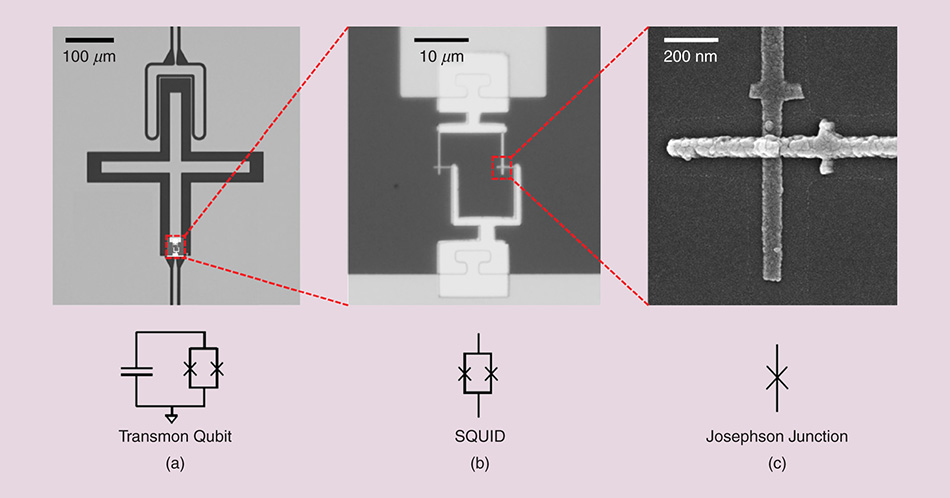
\includegraphics[width=1\textwidth]{images/quanten-hardware/Transmon Qubit.jpg}
    \caption{(a) vollständiges Qubit, (b) Zoom auf die SQUID-Schleife, (c) Josephson-Kontakt}
    \label{fig:transom_image}
    \end{figure}

\subsubsection{Ein-Qubit-Gatter}
Ein-Qubit-Gatter sind die grundlegendsten Operationen in einem Quantencomputer und ermöglichen die gezielte Manipulation des Zustands eines einzelnen Qubits.Diese Gatter, die Rotationen auf der Bloch-Kugel darstellen (z.B. X-, Y- und Z-Rotationen), werden in supraleitenden Quantencomputern durch die präzise Anwendung von Mikrowellenpulsen realisiert.
\\\\
Ein-Qubit-Gatter werden durch das Anlegen von Mikrowellenpulsen realisiert, die auf die Übergangsfrequenz des Qubits abgestimmt sind. Diese Pulse induzieren kohärente Oszillationen, sogenannte Rabi-Oszillationen, zwischen den \big \vert0⟩ und \big \vert1⟩ Zuständen des Qubits. Die Dauer und Phase dieser Pulse bestimmen die Art der Rotation auf der Bloch-Kugel. Beispielsweise können X- und Y-Rotationen durch entsprechend phasenverschobene Mikrowellenpulse erzeugt werden. Z-Rotationen können oft virtuell durch Software implementiert werden, indem die Phase der nachfolgenden Mikrowellenanregungen angepasst wird, was keine physische Pulsdauer erfordert (Characterizing Superconductiong Qubits).\\\\Der Signalpfad für die Qubit-Steuerung ist eine komplexe Kette, die von Raumtemperatur-Elektronik bis zum Qubit im Dilutionskühler reicht. Die Erzeugung der präzisen Mikrowellenpulse beginnt bei Raumtemperatur mit Arbitrary Waveform Generators (AWGs) und Digital-Analog-Wandlern (DACs), die die Basisband-Pulswellenformen erzeugen. Diese Basisband-Signale werden dann mittels Mischer mit einem lokalen Oszillator (LO) zu Mikrowellenfrequenzen (typischerweise 2-10 GHz) hochkonvertiert (Bao Zenghui, 2024). Die Mikrowellensignale werden über Koaxialkabel durch die verschiedenen Temperaturstufen des Kryostaten (z.B. 3K, 1K, 100mK, 10mK) zum Qubit geleitet. Entlang dieses Pfades sind Dämpfungsglieder und Filter angebracht, die an den jeweiligen Temperaturstufen thermisch verankert sind. Ihre Funktion ist es, das von Raumtemperatur eindringende Rauschen zu reduzieren und unerwünschte Frequenzen zu unterdrücken, die die Qubit-Kohärenz stören könnten. Am kältesten Punkt (mK-Stufe) erreichen die Signale den Qubit-Chip über On-Chip-Drive-Lines, die kapazitiv oder induktiv mit den Qubits gekoppelt sind. Die Skalierung dieser Verkabelung stellt eine erhebliche Herausforderung dar, da jede zusätzliche Leitung Wärme in den Kryostaten einbringt und die Kühlleistung begrenzt ist. Dies treibt die Forschung an monolithisch integrierter Steuerungselektronik direkt auf dem Qubit-Chip voran, um den Verkabelungsaufwand und die Wärmelast zu reduzieren (Bao Zenghui, 2024).

\subsubsection{Zwei-Qubit-Gatter}
Zwei-Qubit-Gatter sind für die Durchführung komplexer Quantenalgorithmen unerlässlich, da sie die Verschränkung von Qubits ermöglichen. Ihre Implementierung erfordert eine kontrollierte Wechselwirkung zwischen den Qubits, die auf verschiedene Weisen hardwareseitig realisiert werden kann. Die Entwicklung der Zwei-Qubit-Kopplung hat sich von direkten zu vermittelten, dynamisch steuerbaren Interaktionen entwickelt, um Skalierungs- und Fehlerreduktionsanforderungen zu erfüllen.\\\\
\textbf{Kapazitive Kopplung:}\\
Die kapazitive Kopplung ist eine grundlegende Methode zur Realisierung von Zwei-Qubit-Gattern. Sie wird physisch durch die Platzierung von leitenden Strukturen (Pads oder \grqq{}Coupler Arms\grqq{} ) in unmittelbarer Nähe der Qubits auf dem Chip erreicht, wodurch eine elektrische Kopplung entsteht. Häufig werden hierfür interdigitierte Kondensatoren oder direkte Pads verwendet, die eine effektive Kapazität zwischen den Qubits herstellen.\\
Eine Herausforderung bei der direkten kapazitiven Kopplung in größeren Systemen ist das unerwünschte Übersprechen (Crosstalk) zwischen nicht benachbarten Qubits, das die Gatter-Fidelität beeinträchtigen kann. Um dies zu mindern, wurden fortgeschrittene Designs entwickelt, die \grqq{}Waveguide Extenders\grqq{} oder \grqq{}Coupler Arms\grqq{} mit interdigitierten oder Gap-Kondensatoren nutzen, um die Kopplung über größere physische Distanzen zu vermitteln und gleichzeitig das Übersprechen zu reduzieren. Diese Extender ermöglichen eine flexiblere Platzierung der Qubits auf dem Chip und schaffen Raum für zusätzliche Komponenten wie Ausleseresonatoren und Purcell-Filter.
\\\\
\textbf{Resonatorbasierte Kopplung (Quantenbus):}\\
Eine weit verbreitete und skalierbare Technik zur Kopplung mehrerer Qubits ist die Verwendung eines Mikrowellenresonators als "Quantenbus". Dieser Resonator fungiert als Vermittler und ermöglicht es Qubits, miteinander zu interagieren, selbst wenn sie nicht direkt benachbart sind. Die Interaktion erfolgt über den Austausch virtueller Photonen mit dem Resonator. Dieses Konzept wird als "Circuit QED" (Quantenelektrodynamik in Schaltkreisen) bezeichnet, analog zur optischen Kavität-QED.\\
Durch gezieltes Abstimmen der Qubits in und aus der Resonanz mit dem Bus können verschränkende Zwei-Qubit-Gatter wie Controlled-NOT (CNOT) oder iSWAP implementiert werden. Der Quantenbus bietet eine effektive All-to-All-Konnektivität zwischen einer Gruppe von Qubits, was für bestimmte Algorithmen vorteilhaft ist. Die "Quantum Bus"-Architektur ist nicht nur ein Kopplungsmechanismus, sondern eine grundlegende architektonische Wahl, die flexible und höhergradige Konnektivität zwischen Qubits ermöglicht. Diese Modularität ist entscheidend für die Entwicklung von Quantenprozessoren, die an spezifische Algorithmen und Fehlerkorrekturcodes angepasst werden können, wodurch die Einschränkungen von festen Topologien und spärlicher Konnektivität in größeren Quantensystemen direkt angegangen werden.

\subsection{Beispiele supraleitende Qubits}
** geplant ist hier die Prozessoren Google Scaymore und IBM Eagle vorzustellen. Muss nochmal abgesprochen werden mit Kapitel 1.7, dass dort keine Überschneidungen entstehen**
\subsection{Herausforderungen supraleitende Qubits}
**Einleitungsabsatz zu den Herausforderungen von supraleitenden Quantencomputern**
\\\\
Der Betrieb supraleitender Qubits erfordert extrem niedrige Temperaturen, typischerweise unter 15 Millikelvin (mK), um die Kohärenz aufrechtzuerhalten und die Supraleitung zu ermöglichen.(The ultimate Guide to Superconducting Quantum Computers, 2025). Diese Bedingungen werden durch spezialisierte Kühlsysteme, hauptsächlich Verdünnungskryostate, erreicht. Innerhalb eines Verdünnungskryostat befinden sich die Qubits auf der kältesten Stufe (~10 mK), während die Mikrowellenelektronik auf höheren Temperaturstufen (1 K, 4 K) angeordnet ist. (What Is Cryogenic Quantum Computing and Why It Matters, 2025). Umfassende Abschirmung und Filterung sind entscheidend, um elektromagnetische Interferenzen zu verhindern und thermisches Rauschen zu unterdrücken, das die fragilen Quantenzustände stören und Dekohärenz verursachen kann. Die kryogene Umgebung ist somit nicht nur ein passives Kühlsystem, sondern eine aktive und komplexe Infrastruktur, die die empfindlichen Quantenzustände grundlegend ermöglicht und schützt. Ihre Rolle geht über die reine Kühlung hinaus, da sie aktiv die notwendige Quantenkohärenz aufrechterhält, indem sie verschiedene Formen von Umgebungsrauschen (thermisch, elektromagnetisch) mindert. Verdünnungskryostate sind spezialisierte kryogene Geräte, die die einzigartigen Eigenschaften eines Gemischs aus den Helium-Isotopen Helium-3 und Helium-4 nutzen, um kontinuierlich Temperaturen von bis zu 2 mK zu erreichen. Historisch gesehen wurden "nasse" Verdünnungskryostate verwendet, die eine kontinuierliche Versorgung mit flüssigem Helium zur Vorkühlung benötigten. Diese Systeme waren effektiv, aber mit hohen Betriebskosten und logistischem Aufwand verbunden. Seit etwa 2010 hat sich ein signifikanter Wandel hin zu kryogenfreien ("trockenen") Systemen vollzogen. Diese trockenen Systeme verwenden geschlossene Pulskühlröhren (Pulse Tube Refrigerators, PTRs) zur Vorkühlung auf etwa 4 K, wodurch die Notwendigkeit einer externen Flüssigheliumversorgung entfällt. Der Übergang zu kryokogenfreien Verdünnungskryostaten ist nicht nur im Trend sondern auch strategisch notwendig für die Skalierung von Quantencomputern. Trockene Systeme bieten kontinuierlichen Betrieb und eliminieren die Notwendigkeit des Nachfüllens von Flüssighelium, was längere und unterbrechungsfreie Quantenexperimente ermöglicht und die Betriebseffizienz erhöht. Allerdings geht dieser Vorteil oft mit erhöhten mechanischen Vibrationen von den Pulskühlern einher. Trotz dieser Vibrationsherausforderung ist der Wechsel zu trockenen Systemen für die Skalierbarkeit unerlässlich, da er längere, unterbrechungsfreie Experimente ermöglicht und die Betriebseffizienz für größere Quantensysteme verbessert. Die Hersteller investieren daher stark in Vibrationsdämpfungstechniken, um diesen Nachteil zu mindern(J.Rothe, 2025).
\\\\
Aktuelle Branchenführer verwenden unterschiedliche Kühlsysteme von verschiedenen Anbietern um die individuellen Anforderungen zu erfüllen. IBM hat sich für das im Dezember 2023 erste modulare Quantencomputer System für das Kühlsystem "KIDE Cryogenic Platform" von dem finnischen Unternehmen Bluefors entschieden. Dieses System ist ein kroykogenfreies System, dass auf die Verbindung mehrere Prozessoren ausgelegt ist. Hier wird der von IBM gesetzte Fokus auf skalierbare und modulare Systeme deutlich. Um die reißige Anzahl an Qubits kühlen zu können werden hier neun Pulskühlröhren verwendet, die dafür sorgen verschiedene Temperaturstufen versorgen zu können (Bluefors, 2023). Durch die Nutzung von Pulskühlröhren anstelle von flüssigem Helium können dabei Kühlzeiten von bis zu 3 Jahren realisiert werden. Um modular zu bleiben, wurde KIDE als hexagonale Kammer mit Zugangstüren für Wartung und Möglichkeiten mehrere Cryostat-Einheiten zu koppeln konzipiert. (IBM Quantum, 2024). Ergänzend arbeitet IBM aktuell an dem Goldeye-Projekt mit dem Ziel eine "Super-Kühlschrank" mit 1,7 Kubikmetern Volumen zu entwickeln um zukünftig größere Quantensysteme kühlen zu können. (Pat Gumann, Jerry Chow, 2022) \cite{gumann_ibm_2022}

Google und Intel setzen ebenfalls auf kryogene Plattformen von Bluefors um ihre supraleitenden zu betreiben \cite{noauthor_cryogenic_2025}(Cryogenic Quantum Hardware: The Cold Engine of Quantum Tech, 2025). **Weiteres Ausführen zu Google und Intel **
\\\\
** Hier muss noch auf Verkabelung und Skalierbarkeit eingegangen werden**
\subsection{Ausblick und Weiterentwicklung}

**Hier kommen inhaltlich Punkte zur Verbesserung von Kohärenzzeiten und Gatterfidelity sowie Miniaturisierung

\section{Quantencomputer aus Ionenfallen-Qubits}
\subsection{Gatterimplementierung}

    \begin{itemize}
        \item Wie funktioniert ein Logischer Gatter bei Ionenfallen-Quantencomputern?
        \item Ein-Qubit-Gatter
        \item Zwei-Qubit-Gatter
        \item Cirac-Zoller-Gatter
        \item Mølmer-Sørensen-Gatter
    \end{itemize}
\subsection{Verwendungsbereiche und Merkmale der Ionenfallen-Qubits}
    \begin{itemize}
        \item Stand der Technologie
        \item Ionenfallen in Quantensimulation und Metrologie
        \item Ionenfallen in Quantencomputer
        \item Wie ist ein Ionenfallen Quantencomputer aufgebaut?
        \item Wie und unter welchen Bedingungen wird ein Ionenfallen Quantencomputer benutzt/verwaltet?
    \end{itemize}
\subsection{Herausforderungen und technische Limitationen}
    \begin{itemize}
        \item Warum gibt es die aktuellen Probleme?
        \item Skalierbarkeit
        \item Gatterzeit
        \item Potenzial
        \item Ansätze zur Lösung aktueller Limitationen: z. B. Quantum Networking
    \end{itemize}

\section{Quantencomputer auf Basis diamantbasierter Qubits (NV-Zentren)}
\subsection{Physikalisches Prinzip}
    \begin{itemize}
        \item Zwei-Niveau-System: Elektronenspins von Stickstoff-Fehlstellen (NV-Zentren) im Diamantgitter
        \item Optische Kontrolle
        \item Mikrowellensteuerung
        \item Kernspins
    \end{itemize}
\subsection{Gatterimplementierung}
    \begin{itemize}
        \item Ein-Qubit-Gatter
        \item Zwei-Qubit-Gatter
    \end{itemize}
\subsection{Verwendungsbereiche und Merkmale der diamantbasierten Qubits}
    \begin{itemize}
        \item Stand der Technologie
        \item Anwendungen
        \item Systemaufbau
        \item Betriebsbedingungen
    \end{itemize}
\subsection{Herausforderungen und technische Limitationen}
    \begin{itemize}
        \item Warum gibt es die aktuellen Probleme?
        \item Skalierbarkeit
        \item Gatterzeiten:
        \item Potenzial und Ansätze:
    \end{itemize}



\section{Titel tbd}
\subsection{Photonische Quantencomputer}
    \begin{itemize}
        \item Grundlegende Prinzipien und Qubit-Kodierung
        \item Schlüsselkomponenten: Photonenerzeugung, -manipulation und -detektion
        \item Vorteile und spezifische Herausforderungen
        \item Aktueller Stand, jüngste Fortschritte (2024-2025) und Ausblick
        \item Engineering- und Skalierungslösungen
        \item Quantenfehlerkorrektur
    \end{itemize}

\subsection{Halbleiterbasierte Qubits: Spin qubits}
    \begin{itemize}
        \item Physikalische Realisierung in Halbleitern
        \item Kontroll- und Auslesemechanismen
        \item Vorteile und spezifische Herausforderungen
        \item Aktueller Stand, jüngste Fortschritte (2024-2025) und Ausblick
        \item Engineering- und Skalierungslösungen
        \item Quantenfehlerkorrektur
    \end{itemize}

\subsection{Neutralatom-Quantencomputer}
    \begin{itemize}
        \item Prinzipien: Atomkühlung, Fallen und Qubit-Kodierung
        \item Steuerung und Auslesung mittels Lasertechnologie
        \item Vorteile und spezifische Herausforderungen
        \item Aktueller Stand, jüngste Fortschritte (2024-2025) und Ausblick
        \item Engineering- und Skalierungslösungen
        \item Quantenfehlerkorrektur
    \end{itemize}

\subsection{Topologische Qubits}
    \begin{itemize}
        \item Theoretische Konzepte: Nichtabelsche Anyonen und Majorana-Fermionen
        \item Ansätze zur Realisierung und Manipulation
        \item Potenzial für inhärente Fehlertoleranz und aktuelle Herausforderungen
        \item Aktueller Stand, jüngste Fortschritte (2024-2025) und Ausblick
        \item Engineering- und Skalierungslösungen
        \item Quantenfehlerkorrektur (über den inhärenten Schutz hinaus)
    \end{itemize}



\section{Quantencomputer-Architekturen und Vernetzung}
Dieses Kapitel widmet sich den physischen Architekturen von Quantenprozessoren und des aufstrebenden Feldes der Quantennetzwerken. Es wird auf den Aufbau von Qubit-Arrays und die Mechanismen ihrer Kopplung eingegangen, die für kohärente Operationen unerlässlich sind. Darüber hinaus werden die strategischen Ansätze zur Skalierung von Quantensystemen durch modulare und verteilte Architekturen beleuchtet, wobei die entscheidende Rolle von Quanten-Interkonnektoren im Mittelpunkt steht. Ein weiterer Schwerpunkt liegt auf der unterstützenden Infrastruktur, einschließlich Kryo- und Hochfrequenzelektronik sowie fortschrittlichen Rauschunterdrückungstechniken, die für den stabilen Betrieb von Quantenhardware unerlässlich sind. Abschließend werden die Konzepte und Technologien erster Quantennetzwerke erörtert, die die Grundlage für ein zukünftiges Quanteninternet bilden. Dieses Kapitel verdeutlicht, dass die Überwindung von Skalierungsbeschränkungen für die Beherrschung der Quantenkommunikation benötigt wird.
\subsection{Aufbau eines Quantenprozessors: Qubit-Array, Kopplungsmechanismen}
Dieser Abschnitt befasst sich mit den grundlegenden physikalischen Realisierungen von Quantenprozessoren, wobei ihre räumliche Anordnung in Arrays und die  Mechanismen, die ihre kohärente Interaktion ermöglichen, beschrieben werden.
\subsubsection{Qubit-Array-Architekturen: Vielfalt und Skalierungsherausforderungen}
Quantenprozessoren arbeiten grundlegend anders als klassische Systeme, indem sie Qubits nutzen, die Superposition und Verschränkung für die Berechnung verwenden. (Quelle 1) Die Architektur muss diese Quantenprinzipien berücksichtigen, und verschiedene physikalische Implementierungen von Qubits werden aktiv erforscht, wobei jede einzigartige Eigenschaften und Skalierungsherausforderungen aufweist. (Quelle 1)
Derzeit werden Supraleitende Qubits, Ionenfallen Qubits, Silizium Spin Qubits, und Topologische Qubits im Bezug auf die Skalierbarkeit erforscht. Diese physikalischen Implementierungen wurden bereits vorangegangen in Kapitel 3 erläutert. Die Diskussion der verschiedenen Qubit-Plattformen – supraleitend, Ionenfallen, Silizium-Spin und topologisch – offenbart einen grundlegenden Aspekt im Design von Quantenprozessoren. Es gibt Kompromisse bei der Optimierung für Skalierbarkeit. Jede Plattform bietet spezifische Vorteile, wie die hohe Qubit-Anzahl bei Supraleitern, die langen Kohärenzzeiten bei Ionenfallen, die CMOS-Kompatibilität von Silizium-Qubits oder die  Fehlertoleranz topologischer Qubits. Gleichzeitig wird für jede Plattform ein spezifisches Skalierungsproblem deutlich. Bei supraleitenden Systemen sind dies beispielsweise kryogene Beschränkungen und die Verdrahtungsdichte. Bei Ionenfallen die individuelle Adressierung und der Aufwand durch Ionen-Shuttling. Bei Silizium-Qubits Rauschen und bei topologischen Qubits der Reifegrad der experimentellen Umsetzung.1 Dies verdeutlicht, dass die Verbesserung einer wünschenswerten Eigenschaft, wie etwa der Kohärenzzeit, oft zu neuen oder verstärkten Herausforderungen in anderen Bereichen führt, wie der Skalierbarkeit, der Komplexität der Steuerung oder der thermischen Last. Die Wahl einer Architektur ist daher keine Suche nach dem "besten" Qubit-Typ, sondern erfordert eine sorgfältige Abwägung dieser Kompromisse im Hinblick auf die angestrebte Skalierungsstrategie und die erforderliche Fehlertoleranz. Dies führt zu der Erkenntnis, dass die Zukunft der Quantenprozessoren wahrscheinlich nicht von einem einzigen dominierenden Qubit-Typ geprägt sein wird, sondern von hybriden Ansätzen oder spezialisierten Architekturen, die auf spezifische rechnerische Aufgaben zugeschnitten sind. Der Fokus verschiebt sich von der bloßen Erhöhung der Qubit-Anzahl hin zur Schaffung von qualitativ hochwertigen, miteinander verbundenen Qubits. Dies erfordert eine ganzheitliche Betrachtung des Systems, bei der die Interaktionen zwischen den Qubits und ihrer Umgebung von Anfang an im Design berücksichtigt werden.
Die folgende Tabelle fasst die Merkmale und Herausforderungen der verschiedenen Qubit-Architekturen zusammen:
\begin{table}[h]
  \centering % Zentriert die Tabelle innerhalb der table-Umgebung
\begin{tabular}{ |p{2,5cm}|p{3,5cm}|p{3cm}|p{3cm}|p{1cm}|  }
 \hline
 \textbf{Qubit Typ}& \textbf{Kopplungsmechanismus} & \textbf{Hauptvorteil} & \textbf{Herausforderung} & \textbf{Quelle}\\
 \hline
 \textbf{Supraleitend}   & Abstimmbar/Parametrisch, Fest    & Hohe Qubit-Anzahl, etablierte Fertigungsprozesse, schnelle Gatter & Kryogene Anforderungen, Verdrahtungsdichte, thermische Last, Übersprechen & 1\\
 \hline
  \textbf{Ionenfallen}   & Laser-vermittelt, Ionen-Shuttling    & Hohe Fidelity, lange Kohärenzzeiten, universelles Gatter-Set & Skalierbarkeit (Einzel-Falle), Ionen-Shuttling-Overhead, Adressierung in großen Arrays & 1\\
 \hline
  \textbf{Silizium Spin}   & Elektrisch (Gate-Steuerung)    & Kompatibilität mit Halbleiterindustrie, Potenzial für Millionen Qubits & ntegration von Auslese/Steuerung, Rauschen, Übersprechen, Resonator-Ringing & 3\\
 \hline
   \textbf{Topologisch}   & Topologische Eigenschaften (z.B. Majorana-Nullmoden)    & Intrinsische Fehlertoleranz, Robustheit gegenüber Umgebungsrauschen & Experimenteller Reifegrad, Komplexität der Realisierung & 1\\
 \hline

 \hline
\end{tabular}
\end{table}
\subsubsection{Kopplungsmechanismen: Von fest zu parametrisch und Sonstige}
Effiziente und hochfidele Kopplungsmechanismen sind von entscheidender Bedeutung, um Wechselwirkungen zwischen Qubits zu vermitteln, Zwei-Qubit-Gatteroperationen zu ermöglichen und Dekohärenzfehler zu minimieren.15
Feste Kopplung: In frühen Experimenten mit supraleitenden Qubits wurde häufig eine feste Kopplung verwendet, die typischerweise durch Kondensatoren vermittelt wurde.18 Obwohl für kleine Systeme effektiv, erweist sich diese Strategie als schwierig auf eine große Anzahl von Qubits zu skalieren, da sie zu unerwünschtem Übersprechen und eingeschränkter Flexibilität führt.18
Abstimmbare und Parametrische Kopplung: Moderne Architekturen setzen zunehmend auf abstimmbare oder parametrisch angesteuerte Koppler.5 Diese Koppler ermöglichen eine selektive Aktivierung von Wechselwirkungen zwischen Qubits, wodurch Übersprechen und umgebungsbedingte Dekohärenz reduziert werden können.16 Parametrische Wechselwirkungen können eine Reihe von Operationen ausführen, darunter Zwei-Qubit-Gatter (z.B. Controlled-Z-Gatter mit einer Fidelity von 98,3), Reset-Operationen, Leckage-Wiederherstellung und das Auslesen von Qubits, alles mit einem einzigen abstimmbaren Koppler. Dies reduziert die Systemkomplexität und den Steueraufwand in skalierbaren Quantenprozessoren erheblich.15 Sie ermöglichen zudem schnelle Zwei-Qubit-Operationen und können mit hoher Geschwindigkeit und einem hohen Ein/Aus-Verhältnis ein- und ausgeschaltet werden.18 Eine Herausforderung besteht jedoch darin, dass das Erreichen einer starken Kopplung zu Qubits unbeabsichtigt die Kohärenz reduzieren kann, was einen Kompromiss darstellt.17 Resonante Einzel-Qubit-Operationen können langsam sein und erfordern große Ansteueramplituden, was in dichteren Schaltungen zu übermäßigem Übersprechen führen kann.20
Metasurfaces für polychromatische Kopplung: Ein innovativer Ansatz beinhaltet kryogen-kompatible Metasurfaces, die eine einzelne Eingangsfrequenz in mehrere gezielte Frequenzen umwandeln und so eine polychromatische Qubit-Kopplung ermöglichen.16 Diese Technologie mindert Übersprechen und umgebungsbedingte Dekohärenz, verlängert die Kohärenzzeiten und bewahrt die Fidelity des Quantenzustands, wodurch komplexe Operationen wie Multi-Qubit-Verschränkung und Fehlerkorrektur unterstützt werden.16
Steuerung von Kopplung und Rauschen: Das komplexe Zusammenspiel von Gerätearchitektur und Leistung mit Qubit-Steuerungsschemata, Erwärmung und Übersprecheffekten ist eine große Herausforderung.10
Die Entwicklung von Kopplungsmechanismen in Quantenprozessoren wird von einem grundlegenden Trilemma geprägt: dem "Steuerung-Kohärenz-Übersprechen"-Problem. Feste Kopplungsmechanismen, obwohl einfach zu implementieren, sind für große Qubit-Anzahlen nicht skalierbar, da sie zu unkontrollierbarem Übersprechen führen.18 Abstimmbare und parametrische Kopplung bieten hier eine deutlich verbesserte Kontrolle und Flexibilität, indem sie selektive Wechselwirkungen ermöglichen und den Steueraufwand reduzieren.15 Die Notwendigkeit schneller Gatteroperationen erfordert jedoch oft starke Ansteuerungen, die paradoxerweise die Qubit-Kohärenz reduzieren können 17 und in dichten Qubit-Arrays zu unerwünschtem Mikrowellen-Übersprechen führen.20 Die Einführung von Lösungen wie kryogen-kompatiblen Metasurfaces, die polychromatische Kopplung ermöglichen, oder die präzise Gestaltung von Steuerpulsen, um Resonanzüberlappungen zu vermeiden, sind Versuche, dieses Trilemma zu navigieren.10 Es geht hierbei nicht nur um die Verbesserung einzelner Komponenten, sondern um die Optimierung der systemweiten Interaktion, um sicherzustellen, dass Verbesserungen in einem Bereich nicht zu einer katastrophalen Verschlechterung in einem anderen führen. Dies erfordert ein tiefes Verständnis der physikalischen Wechselwirkungen und eine präzise technische Umsetzung. Diese Entwicklung deutet darauf hin, dass die zukünftige Entwicklung von Quantenprozessoren stark auf einem integrierten Co-Design von Qubit-Arrays und ihren Steuerungs- und Kopplungsmechanismen basieren wird, das über die isolierte Komponentenoptimierung hinausgeht. Dies erfordert ausgefeilte Simulations- und Fertigungstechniken, um komplexe Interaktionseffekte vorherzusagen und zu mindern. Die Fähigkeit, diese Kompromisse effektiv zu managen, wird die Skalierbarkeit und Leistungsfähigkeit zukünftiger Quantencomputer maßgeblich bestimmen.

\subsection{Skalierungsstrategien: Modulare Systeme}
\subsection{Unterstützende Infrastruktur: Kryo-Elektronik, Hochfrequenzelektronik, Steuerungseinheiten, Filter gegen thermisches Rauschen}
\subsection{Erste Netzwerke: Konzepte des Quanteninternets (Architekturmodell), Quantenrepeater, Quantenrouter, Verschränkungsverteilung}

\section{Praxisbeispiel(e): Im Inneren eines IBM-Quantencomputers}
Die Entwicklung kommerziell nutzbarer Quantencomputer stellt eine der größten wissenschaftlichen und ingenieurtechnischen Herausforderungen unserer Zeit dar. Während die physikalischen Grundlagen der Quantenmechanik, wie Qubit-Logik, Superposition und Verschränkung in den vorangegangenen Kapiteln dieses Buches bereits detailliert erläutert wurden, fokussiert sich dieses Kapitel auf die konkrete Hardwarearchitektur und Systemintegration eines der ersten kommerziellen Quantencomputersysteme: das IBM Q System One. Dieses System wurde erstmals 2019 vorgestellt und markiert einen wichtigen Meilenstein im Quantencomputing. IBM Q System One zielt darauf ab, Quantencomputing aus dem reinen Forschungslabor heraus und in eine zuverlässigere, wartungsärmere und industriell einsetzbare Form zu überführen (Gambetta et al., 2019; IBM News Room, 2019).


\subsection{Aufbaus eines kommerziellen Quantencomputers - IBM Q System One}
Beschreibung des Aufbaus eines kommerziellen Quantencomputers - IBM Q System One
Dieser Abschnitt beschreibt die physikalische Struktur eines typischen supraleitenden Quantencomputers. Im Fokus steht der Qubit-Chip, der auf einer stark heruntergekühlten Plattform montiert ist – einer sogenannten Verdünnungskühlstufe mit Temperaturen im Millikelvin-Bereich. Verschachtelte Abschirmungen und Vakuumkammern sorgen für eine minimale Störung durch Wärme, Strahlung oder elektromagnetische Einflüsse von außen.

\subsection{Foto-Illustration}
Foto-Illustration: Kaltes Verdünnungskryostat mit hängender Chip-Ebene (Gold-Coax-Kabel zu Qubits)
Hier wird mithilfe eines Bildes gezeigt, wie ein realer Kryostat aufgebaut ist, in dem der Qubit-Chip „hängt“. Die goldfarbenen Koaxialkabel, die an den Chip führen, dienen der Steuerung und Auslesung der Qubits mit hochfrequenten Mikrowellensignalen. Das Bild veranschaulicht die aufwendige technische Infrastruktur, die notwendig ist, um Quantenoperationen durchzuführen.


\subsection{Erläuterung eines einzelnen supraleitenden Qubits (Transmon)}
Erläuterung eines einzelnen supraleitenden Qubits (Transmon) und wie ein Zwei-Qubit-Gatter durch kapazitive Kopplung realisiert wird
Ein Transmon-Qubit ist ein spezieller supraleitender Schaltkreis, der zur Stabilisierung gegen Ladungsrauschen designt wurde. In diesem Teil wird erklärt, wie durch gezielte Mikrowellenpulse Zustände manipuliert und gelesen werden können. Zusätzlich wird gezeigt, wie zwei Transmon-Qubits über kapazitive Kopplung ein kontrolliertes Quantenlogikgatter bilden – ein zentrales Element zur Realisierung von Quantenalgorithmen.

\subsection{IBM Quantum System Two – Auf dem Weg zur Quanten-zentrierten Supercomputation}
Die Einführung des IBM Quantum System Two, dessen Details erstmals im Dezember 2023 umfassend vorgestellt wurden (Gambetta, 2023; IBM News Room, 2023), signalisiert einen signifikanten Fortschritt durch IBM in der Entwicklung kommerziell verfügbarer Quantencomputersysteme. Dieses System stellt nicht lediglich eine Weiterentwicklung des IBM Q System One dar, sondern verkörpert einen Paradigmenwechsel hin zu einer Architektur, die durch Modularität, Skalierbarkeit und Vernetzbarkeit charakterisiert ist. Diese Architektur soll als Fundament für das Konzept des „Quantum-centric Supercomputing“ dienen.

\subsubsection{Designphilosophie und Architekturziele}
Im Unterschied zum eher monolithischen Aufbau des IBM Q System One, das primär für den Betrieb eines einzelnen Quantenprozessors (QPU) konzipiert war, wurde das IBM Quantum System Two von Grund auf mit Blick auf mehrere Kernziele entwickelt. 

Zu diesen Zielen zählt erstens die Modularität: Das System ist so strukturiert, dass es aus multiplen, potenziell miteinander verbundenen Modulen aufgebaut werden kann. Dieser Ansatz ermöglicht eine flexible Systemkonfiguration und eine schrittweise Erweiterung der Gesamtanlage. Zweitens steht die Skalierbarkeit im Fokus, mit dem Ziel, ein Wachstum auf Tausende von Qubits und darüber hinaus zu ermöglichen. Dies soll durch die Kooperation mehrerer QPUs innerhalb eines oder mehrerer vernetzter Systeme realisiert werden. Drittens ist die Konnektivität von essenzieller Bedeutung für die Skalierbarkeit. Darunter wird die Fähigkeit verstanden, QPUs sowohl innerhalb eines Systems als auch systemübergreifend zu verbinden, um die Bearbeitung umfangreicherer und komplexerer Problemstellungen zu ermöglichen. Viertens wurden Aspekte der Servicefreundlichkeit und Aufrüstbarkeit berücksichtigt; das modulare Design ist darauf ausgelegt, Wartungsarbeiten sowie die Implementierung von Hardware-Upgrades – beispielsweise neue QPU-Generationen oder verbesserte Steuerungselektronik – zu vereinfachen. Fünftens bildet die Hybridität, also die nahtlose Integration mit klassischer Hochleistungsrechner-Infrastruktur, einen zentralen Bestandteil der Vision des Quantum-centric Supercomputing.Kernbestandteil der Vision des Quantum-centric Supercomputing.

\subsubsection{Systemarchitektur und Gehäuse}
Das IBM Quantum System Two weist eine deutlich veränderte äußere Erscheinungsform auf. Die für das System One charakteristische Glaskuppel wurde durch eine umfangreichere, hexagonale Struktur ersetzt. Diese besteht aus hexagonal geformten Basiseinheiten, welche jeweils einen Kryostaten mit Quantenprozessoren sowie die zugehörige unterstützende Infrastruktur aufnehmen können. Die Wahl der hexagonalen Form ist nicht rein ästhetisch motiviert, sondern dient auch funktionalen Zwecken, indem sie die Verbindung mehrerer solcher Einheiten zu größeren Clustern erlaubt (Red Dot Design Award, 2024). Jede dieser Einheiten weist Abmessungen von etwa 4,6 Metern in der Höhe und 6,7 Metern in der Breite auf. Die modulare Erweiterung wird dadurch realisiert, dass an die Seitenflächen dieser hexagonalen Einheiten weitere Module angedockt werden können. Diese zusätzlichen Module können entweder weitere QPUs oder klassische Steuer- und Peripherieelektronik enthalten, was ein physisches Wachstum des Systems parallel zur Steigerung der Rechenleistung ermöglicht. Bei den Materialien und dem Design des Gehäuses kommen eloxiertes, poliertes Aluminium sowie Glaselemente zum Einsatz. Die sichtbaren Fugen zwischen den Modulen akzentuieren den modularen Charakter des Systems (iF Design Award, 2024). Das Gesamtdesign zielt darauf ab, Prinzipien der Offenheit und Zugänglichkeit zu vermitteln, während gleichzeitig der Schutz der sensitiven Technologie gewährleistet wird.

\subsubsection{Kryogene Infrastruktur und QPU-Umgebung}
Die Notwendigkeit, eine steigende Anzahl von Qubits bei extrem tiefen Temperaturen – typischerweise im Bereich von 10 bis 20 Millikelvin für supraleitende Qubits – zu betreiben, stellt hohe Anforderungen an die kryogene Infrastruktur. Im Hinblick auf eine skalierbare Kühlung müssen, obgleich die fundamentalen Prinzipien der Dilutionsrefrigeration beibehalten werden, die Kühlleistung und die interne Kapazität der Kryostaten für das Quantum System Two signifikant erhöht werden. Dies ist erforderlich, um multiple oder größere QPUs sowie die damit assoziierte Verkabelung und Komponenten, wie beispielsweise Verstärker, adäquat zu versorgen. In diesem Kontext hat IBM auch den „Goldeneye“-Kryostaten erwähnt, einen Dilutionsrefrigerator mit einer besonders großen Kühlkapazität, welcher für die Kühlung zukünftiger Generationen von Multi-Chip-Prozessoren ausgelegt ist (SpinQ, 2025). Die Integration von Prozessoren ist ein weiteres Kernelement; Quantum System Two ist dafür konzipiert, mehrere Quantenprozessoren, beispielsweise drei IBM Heron Prozessoren, in einem einzelnen Kryostaten zu beherbergen und zu betreiben (arXiv, 2024). Eine solche Integration erfordert eine präzise Planung der internen Verkabelung, der thermischen Anbindung und der elektromagnetischen Abschirmung. Das Vibrationsmanagement und die Stabilität gewinnen in einem modularen und potenziell sehr ausgedehnten System zusätzlich an Komplexität und Kritikalität im Vergleich zum System One, um die Kohärenz der Quantenzustände sicherzustellen.

\includepdf[pages=1, fitpaper=true]{GrafikKühlungDeutsch.pdf}


\subsubsection{Signalübertragung, Steuerungselektronik und Konnektivität}
Mit der Zunahme der Anzahl von Qubits und Prozessoren steigen die Anforderungen an die Steuerungs- und Ausleseelektronik sowie an die Verbindungen zwischen den Systemkomponenten exponentiell. IBM hat eine Steuerungselektronik der dritten Generation entwickelt, die sich durch eine höhere Kompaktheit, gesteigerte Leistungsfähigkeit und eine engere Integration mit den QPUs auszeichnet. Diese Elektronik ist darauf ausgelegt, eine größere Anzahl von Qubits effizient zu steuern und auszulesen (IBM News Room, 2023). Die Erhöhung der Qubit-Dichte und -Anzahl macht zudem innovative Lösungen für eine hochdichte kryogene Verkabelung notwendig, um die Wärmelast gering zu halten und gleichzeitig eine hohe Signalintegrität zu gewährleisten. Flexible kryogene Hochfrequenzleitungen (CryoFlex) spielen hierbei eine wichtige Rolle. Für die Koordination und das sogenannte „Circuit Knitting“ – ein Verfahren, das große Quantenschaltkreise auf mehrere QPUs aufteilt und klassische Kommunikation von Zwischenergebnissen erfordert – sind leistungsfähige klassische Kommunikationslinks zwischen den Prozessoren und den Steuerungseinheiten unerlässlich. Langfristig verfolgt IBM das Ziel, auch direkte quantenkohärente Verbindungen (Quantum Links) zwischen QPUs zu realisieren, um echte verteilte Quantenberechnungen über mehrere Chips hinweg zu ermöglichen (IBM Quantum Roadmap).

\subsubsection{Integration klassischer und quantenmechanischer Komponenten}
Das IBM Quantum System Two ist als zentrales Element einer „Quantum-centric Supercomputing“-Architektur konzipiert. Dies impliziert, dass das System für eine enge Kooperation mit klassischen Supercomputern und Cloud-Ressourcen ausgelegt ist, um hybride Workflows zu unterstützen. Middleware und Software-Werkzeuge wie Qiskit werden kontinuierlich weiterentwickelt, um solche hybriden Quanten-Klassik-Workflows effizient zu orchestrieren, Rechenaufgaben dynamisch zu verteilen und Ergebnisse zu konsolidieren (The Quantum Insider, 2024). Der Ansatz des Quantum Serverless zielt darauf ab, Quanten- und klassische Berechnungen nahtlos in unterschiedlichen Umgebungen, sei es in der Cloud oder on-premises, zu integrieren und auszuführen.

\subsubsection{Wartung, Skalierbarkeit und Modularität in der Praxis}
Die praktische Umsetzung der Prinzipien von Modularität und Skalierbarkeit stellt einen Hauptfokus bei der Entwicklung des IBM Quantum System Two dar. Das System ist für eine phasenweise Inbetriebnahme (Phased Deployment) und für Upgrades konzipiert. Dies bedeutet, dass es schrittweise ausgebaut und mit neueren Prozessorgenerationen (wie den in der IBM Roadmap genannten zukünftigen Prozessoren Flamingo oder Kookaburra) oder verbesserter Steuerungshardware aufgerüstet werden kann, ohne dass ein Austausch des Gesamtsystems notwendig wird. Das Design berücksichtigt ferner die Notwendigkeit regelmäßiger Wartung durch entsprechend gestaltete Servicezugänge, die den Zugriff auf kritische Komponenten erleichtern. Über spezifische Wartungsprozeduren sind, ähnlich wie beim System One, öffentlich meist nur allgemeine Informationen verfügbar.

\subsubsection{Relevante Designentscheidungen aus Ingenieursperspektive}
Mehrere zentrale Designentscheidungen prägen die ingenieurtechnische Ausrichtung des IBM Quantum System Two. Die Priorisierung der Modularität stellt hierbei die fundamentalste und weitreichendste Entscheidung dar, welche die Skalierbarkeit und Zukunftsfähigkeit des Systems gewährleisten soll. Parallel dazu wurde ein starker Fokus auf die Interkonnektivität gelegt; die Fähigkeit, Prozessoren und Systeme miteinander zu verbinden, ist entscheidend, um die Limitierungen einzelner QPUs zu überwinden. Die Entwicklung des Systems folgt einem integrierten Ansatz, bei dem Hardware, Software (einschließlich Qiskit und Middleware), Steuerung und klassische Computerressourcen als eine kohärente Einheit betrachtet und entwickelt werden. Schließlich schafft die Architektur des Quantum System Two, obwohl sie selbst noch nicht die Ära der vollständigen Fehlertoleranz einläutet, die notwendige Skalierbarkeit und Komplexität, um fortgeschrittene Fehlerminderungs- und Quantenfehlerkorrekturcodes zu implementieren und zu testen.
\\

Das IBM Quantum System Two stellt somit einen entscheidenden Evolutionsschritt dar. Es legt die technologischen Grundlagen für Quantencomputer, die potenziell in der Lage sein werden, Probleme von praktischer Relevanz zu lösen, welche für klassische Supercomputer als unlösbar gelten. Die Realisierung dieser Vision ist maßgeblich von der erfolgreichen Bewältigung der komplexen ingenieurtechnischen Herausforderungen in den Bereichen Skalierung, Konnektivität und Systemintegration abhängig.


\printbibliography
